\section{Introduction}
Bibliographic data sources are organized digital collections of reference metadata and citation links related to published scientific literature. One primary purpose is to assess the scholarly performance, although it is important to exercise caution when employing bibliometric indicators for performance evaluation \citep{van2013scientists, hicks2015bibliometrics, priem2011altmetrics}. Another objective of bibliometric analyzes is science mapping, a process that involves synthesizing extensive data, prioritizing impactful research, and extracting key knowledge structures \citep{chen2017science}. Given the rapid proliferation of scientific publications, science mapping evidence is particularly valuable for reconstructing the theoretical framework of empirical studies or literature reviews.

%Bibliographic databases can be multidisciplinary, (\emph{e.g.}, Web of Science and Scopus), or specialized, (\emph{e.g.}, PubMed, Cochrane, Medline, EconBiz, IEEE Xplore, and Astrophysics Data System). Other analogous databases exist for patent data and digital materials, (\emph{e.g.}, arXiv, DBPL, CiteSeerXPatent). Google Scholar differs from the aforementioned data sources in that it does not permit users to download any metadata \citep{dallas2018variable}.

Recently, new sources of multidisciplinary bibliographic data have emerged, including Microsoft Academic, launched in 2016 \citep{sinha2015overview, wang2019review, wang2020microsoft}, Semantic Scholar launched in 2015 \citep{ammar2018construction}, and CrossRef, an open bibliographic data source launched in 2017 \citep{hendricks2020crossref, van2018crossref}.  Dimensions is a scientometric data source that provides also information on grants, datasets, clinical trials, patents, and policy documents \citep{herzog2020dimensions, hook2018dimensions}. These databases complement the many existing open and commercial sources. The two most widely used commercial multidisciplinary databases are Web of Science and Scopus while the specialized ones include PubMed, EconBiz, and arXiv, which are the main open bibliographic sources for medicine, economics, and physical sciences and engineering, respectively.

The value of these open and commercial bibliographic data sources hinges on several characteristics: (1) document coverage, (2) completeness and accuracy of citation links, (3) update speed, (4) automation of data access through web interfaces, APIs, and data dumps, and (5) the terms of use for a data source \citep{wanyama2022you, kulkanjanapiban2022comparative, singh2021journal, martin2021google, visser2021large, waltman2020special, winter2017rentrez}. OpenAlex is recognized for providing the most extensive coverage of scientific literature, encompassing a notably larger number of documents compared to other data sources (see \href{https://openalex.org/about}{https://openalex.org/about}). Its document coverage outpaces all major databases, including Microsoft Academic \citep{visser2021large, wang2020microsoft} and CrossRef, which are its primary sources. While Google Scholar reportedly boasts an estimated 389 million database, it is crucial to note that Google Scholar does not adhere to the conventional database model due to its lack of comprehensive metadata, and it does not permit users to download query search results \citep{dallas2018variable}. 

Another remarkable strength of OpenAlex is its substantial collection of open-access works, totaling 48 million. This extensive repository grants users open and free access to a wealth of scholarly resources, aligning with OpenAlex's dedication to open science principles. This commitment promotes both accessibility and transparency in the sharing of knowledge. Furthermore, OpenAlex stands out not only in terms of quantity but also in data quality. With a substantial number of citations amounting to 1.9 billion, OpenAlex emphasizes its relevance for researchers engaged in citation-based studies. This robust citation data enhances its appeal as a valuable resource for scholars conducting research reliant on citation analysis.

The purpose of this article is to introduce the OpenAlexR R package, which facilitates the retrieval of metadata from OpenAlex, performs specific functions, and formats the data for utilization in bibliometrix, particularly for science mapping and research assessment purposes.




\subsection{OpenAlex}
Named after the ancient Library of Alexandria, \href{http://docs.openalex.org}{OpenAlex} is a free and fully open catalogue of scholarly metadata with open data, open APIs, open-source code \citep{priem2022openalex}.
Behind this tour de force is OurResearch, a nonprofit organisation dedicated to open principles of academic works with other impactful projects such as CiteAs \citep{du2021citeas} and Unpaywall \citep{chawla2017unpaywall}.
OpenAlex was launched in January 2022, timely replacing the retired Microsoft Academic system. OpenAlex is already extensively used in many scholarly articles \citep{belfiore2022characterising}. 
The data is currently accessible through a complete database snapshot and a \href{https://en.wikipedia.org/wiki/Representational_state_transfer#Applied_to_web_services}{REST API} that is updated daily.

The OpenAlex database consists of eight academic entity types: works, authors, institutions, sources, concepts, publishers, funders, geo (Fig. \ref{oa-metagraph}). It is important to know the OpenAlex entities because it is possible to make query for each entity. In fact, each entity is assigned an OpenAlex ID (OAID) which represents the primary key to access the data. 
However, OpenAlex also recognizes different \href{https://docs.openalex.org/how-to-use-the-api/get-single-entities#canonical-external-ids}{external canonical IDs} for different entities.
We briefly summarise the eight entities below.
For more detail, visit the \href{http://docs.openalex.org/}{documentation page} and the more recent \href{https://docs.openalex.org/download-all-data/upload-to-your-database/load-to-a-relational-database/postgres-schema-diagram}{Postgres schema diagram} by OpenAlex.

\begin{figure}[htbp]
  \centering
  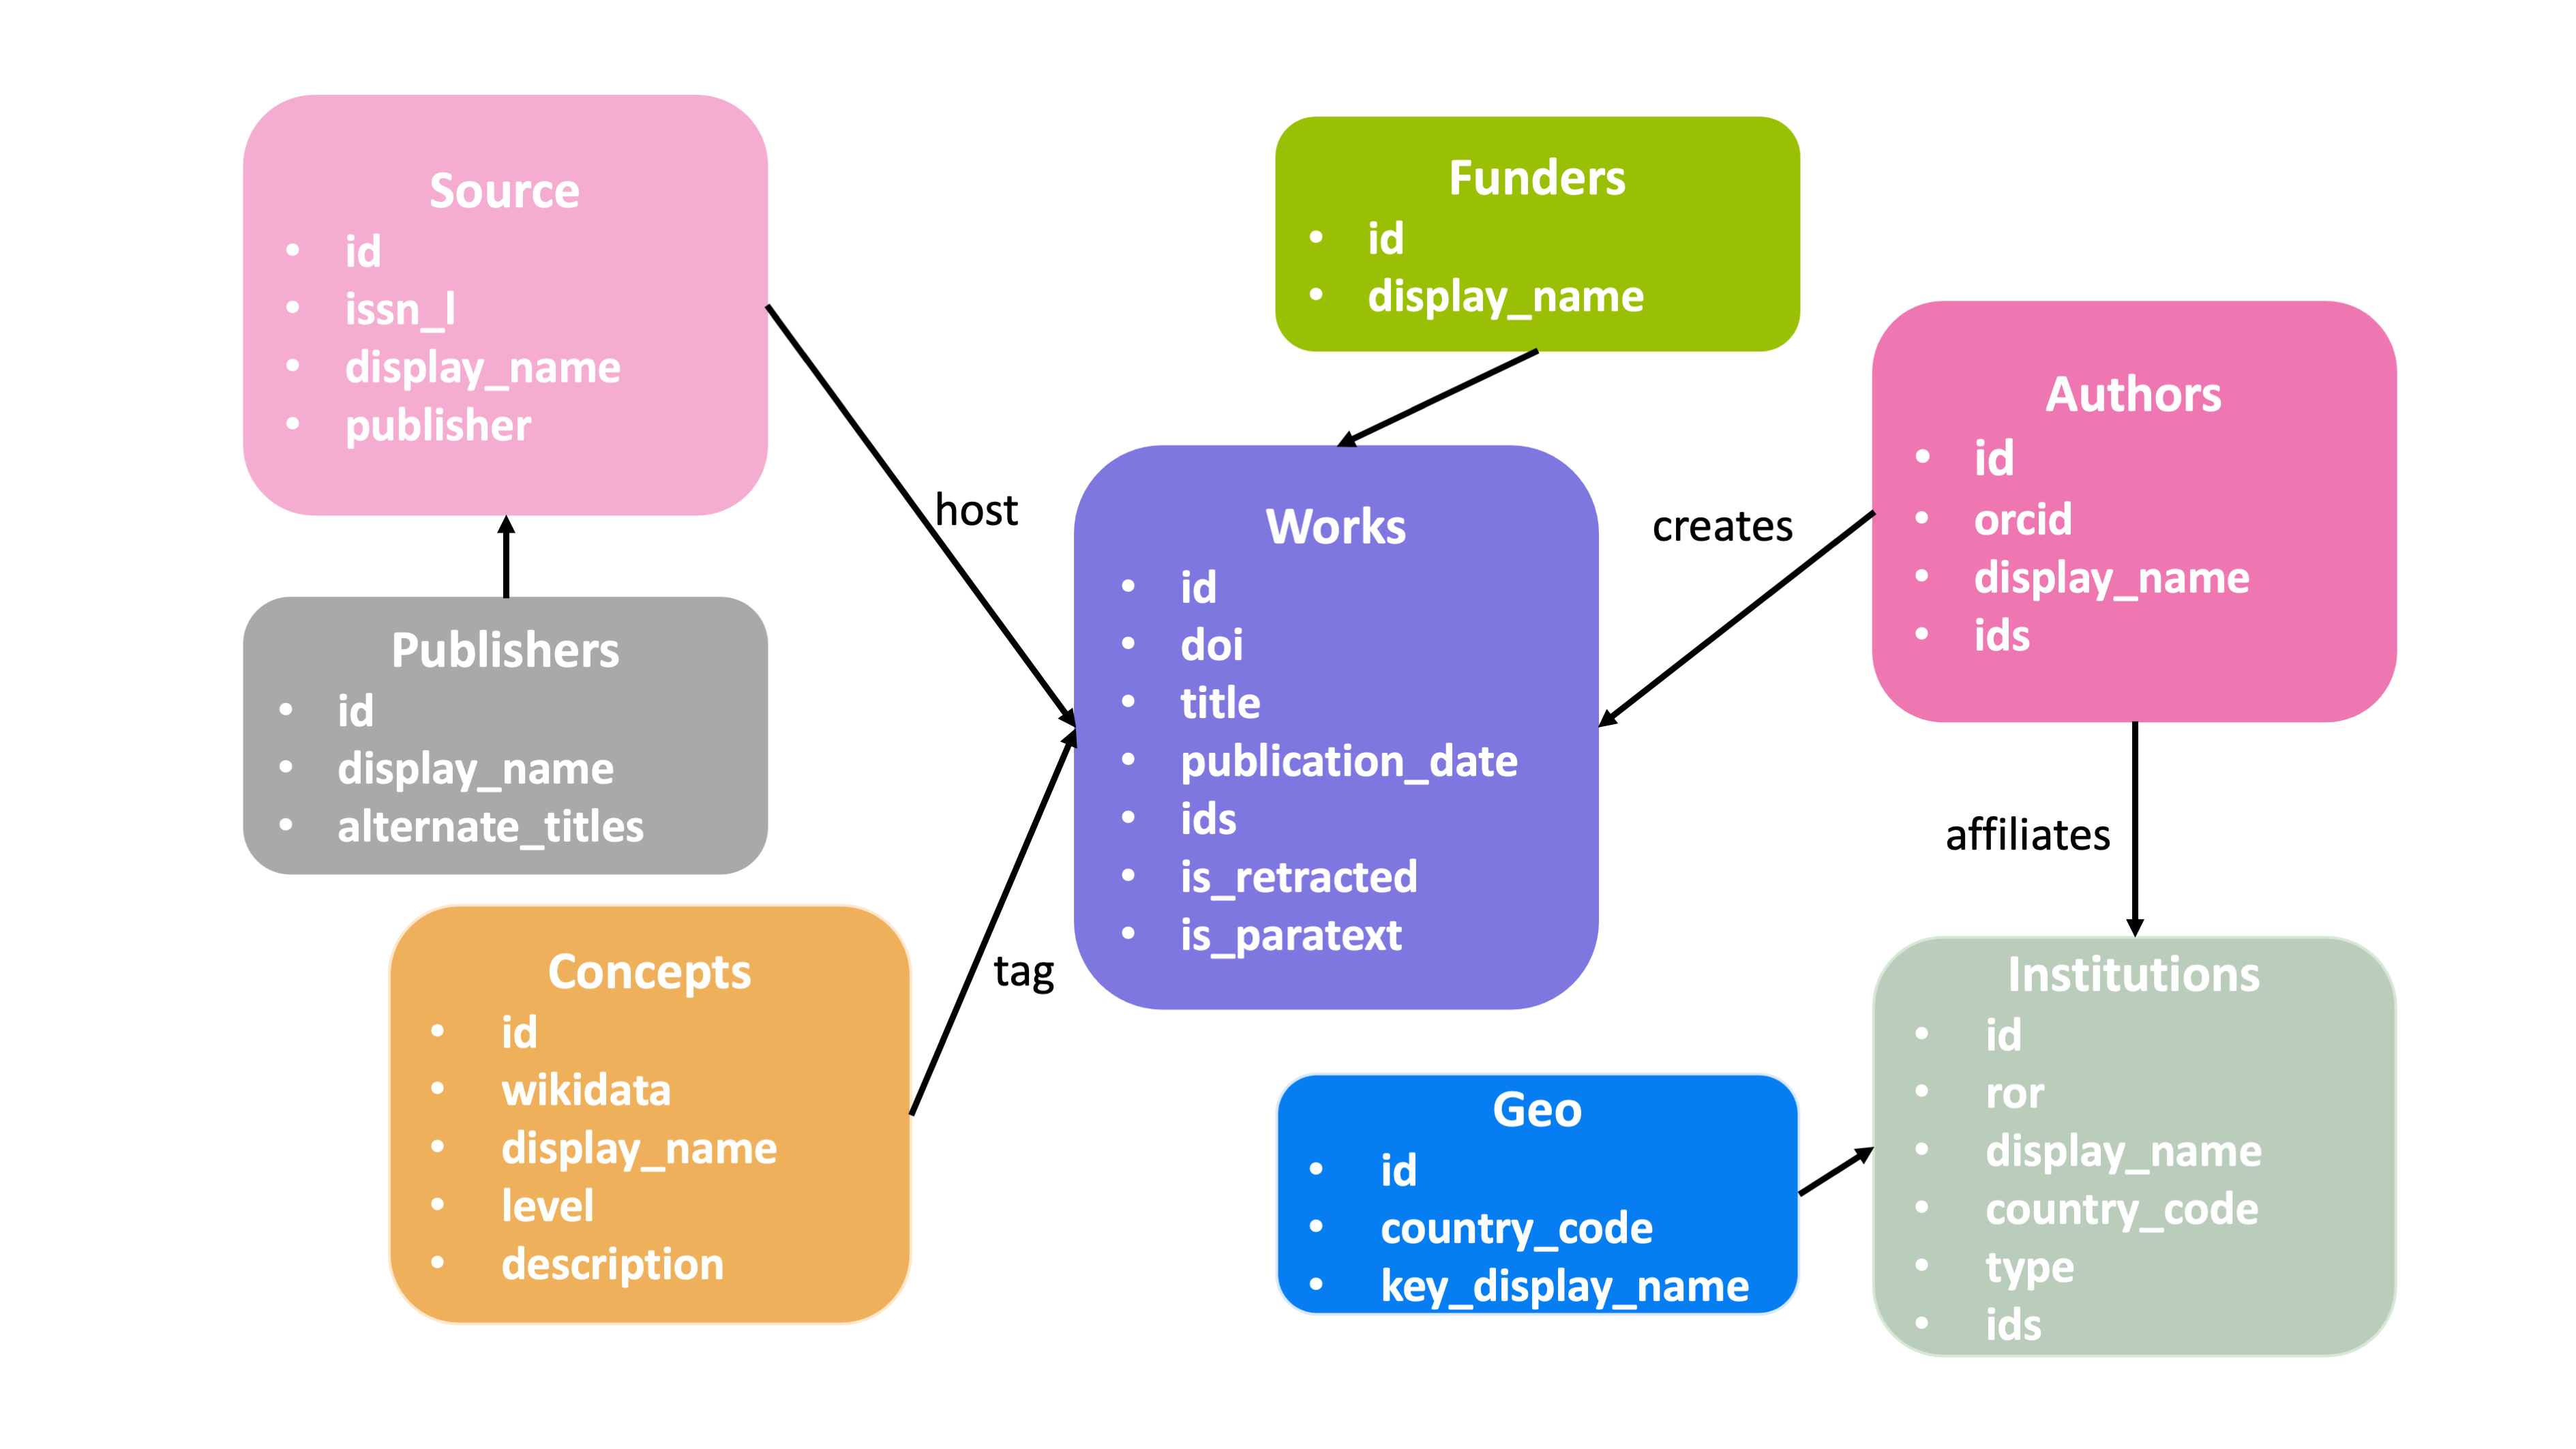
\includegraphics[scale=0.40]{figures/oa-metagraph}
  \caption{Eight OpenAlex entities and their first few attributes.}
  \label{oa-metagraph}
\end{figure}

\begin{itemize}
\item \textbf{Works}: academic documents such as journal articles, proceedings, books, and datasets.
The Works entity is central in that it ties together the other four entities (Fig. \ref{oa-metagraph}).

OpenAlex indexes over 200 million works.
One can identify a work by its OAID or \href{https://www.doi.org/}{DOI}, a unique alphanumeric string assigned to a digital document, often a research article.

\item \textbf{Authors}: individuals who create works.
Authors create Works, study Concepts, and are affiliated with Institutions.
OpenAlex indexes more than 200 million authors.
One can identify an author by their OAID or \href{https://orcid.org/}{ORCID}, a persistent and unique identifier assigned to researchers.

\item \textbf{Institutions}: universities and organisations affiliated with authors.
Institutions are linked to Works via Authors.
OpenAlex indexes more than 100,000 institutions.
One can identify an institution by its OAID or \href{https://ror.org/}{ROR} ID, a persistent identifier for research organizations.

\item \textbf{sources}: repositories that house works such as journals, conferences, preprint repositories, or institutional repositories.
OpenAlex uses a fingerprinting algorithm to match multiple locations a work may be hosted in and flag the version of the record's host as primary.
OpenAlex indexes more than 100,000 sources.
One can identify a source by its OAID or ISSN-L, \emph{i.e.}, a single ISSN that groups the publication's all possible \href{https://www.issn.org/}{ISSNs} (standardized numeric identifiers assigned to serial publications).

\item \textbf{Concepts}: topics of works, deduced from their titles and abstracts.
To identify a concept, you can use the OAID or its \href{https://www.wikidata.org/wiki/Wikidata:Identifiers}{Wikidata ID}, a unique identifier assigned to that entity in Wikidata because all OpenAlex concepts are also Wikidata concepts.
The concepts follow a hierarchy; there are 19 concepts at the root level (0-level) and 5 layers of descendants. 
OpenAlex indexes $\sim$ 65,000 concepts.

\item \textbf{Publishers}: companies and organizations that distribute academic documents. Each publisher publishes multiple journals, so publisher data is aggregate data. OpenAlex indexes about 10,000 publishers.

\item \textbf{Funders}: public and private companies that fund research. OpenAlex indexes about 30,000 funders. Funder data comes from Crossref, and is enhanced with data from Wikidata and ROR.

\item \textbf{Geo}: works produced in the country based on the nationality of the institution with which the author is affiliated. In particular, there are some ways to filter and group academic documents by continents and the Global South. OpenAlex uses United Nations data to divide the globe into continents and regions, making it easier to filter the data.

\end{itemize}



\section{Implementation of openalexR} \label{implementation}

Interacting with the OpenAlex API, \pkg{openalexR} provides easy querying and downloading of scholarly metadata as well as converting the output into a classic bibliographic dataframe (Fig. \ref{oa_workflow}), which allows the user to streamline their data collection and downstream analyses \citep{oaR}.

\begin{figure}[htbp]
  \centering
  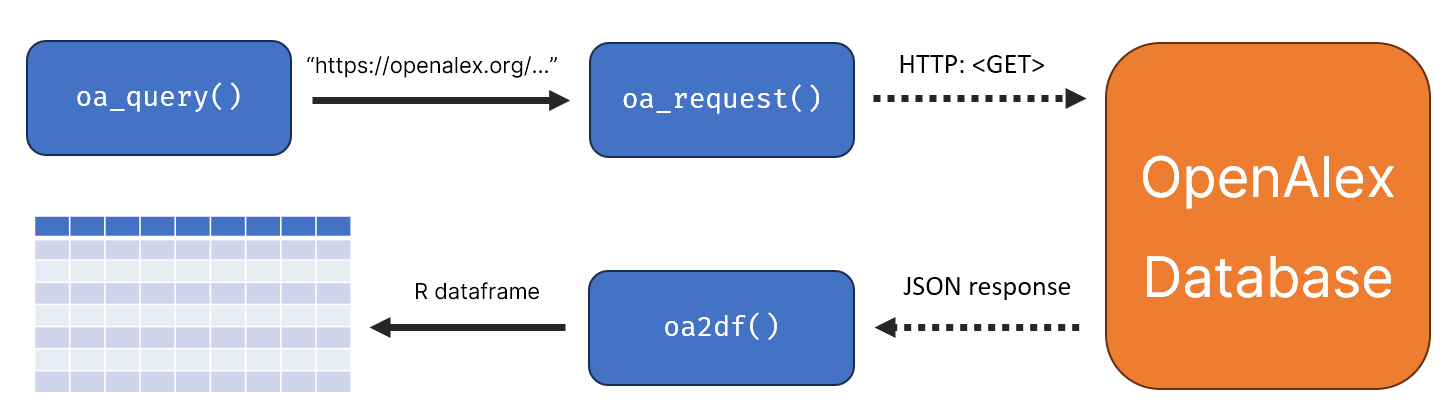
\includegraphics[scale=0.3]{figures/oa_workflow}
  \caption{openalexR workflow}
  \label{oa_workflow}
\end{figure} 

With minimal dependencies, \pkg{openalexR} lowers the barrier to using the \href{https://docs.openalex.org/how-to-use-the-api/api-overview}{REST API} by simplifying input entry, handling rate limits, and automatically parsing API responses.
The package also offers other useful functionality such as snowball search and N-grams of works.
\pkg{openalexR} is currently listed on the \href{https://docs.openalex.org/api#client-libraries}{OpenAlex website} as the supported R library for API access.
The main function of \pkg{openalexR}, \code{oa\_fetch}, is a convenience wrapper for three smaller functions to

\begin{enumerate}
  \item generate a valid query from a set of arguments provided by the user (\code{oa\_query}), 
  \item download a collection of entities matching the query (\code{oa\_request}),
  \item and convert the list output to a classical bibliographic data frame (\code{oa2df}).
\end{enumerate}

Specifically, in constructing valid queries following the OpenAlex API syntax, \code{oa\_query} utilizes the \code{modify\_url} function of the \CRANpkg{httr} package \citep{hadley2022httr} to pass the \code{filter}, \code{sort}, \code{search}, and \code{group\_by} parameters specified by the user.
Next, \code{oa\_request} sends a request to OpenAlex, downloads the JSON output matching the created query, and returns the result in a nested list.
Finally, \code{oa2df} converts this output list into a classic bibliographic data frame (similar to an Excel sheet) that can be used as input in a bibliometric analysis or scientific mapping \citep{wais2016gender}, \emph{e.g.}, using the \CRANpkg{bibliometrix} package \citep{aria2017bibliometrix}. 

In addition to \code{oa\_fetch}, the package \CRANpkg{openalexR} includes three other functions specific to certain features: \code{oa\_random}, \code{oa\_snowball}, and \code{oa\_ngrams}. 
The function  \code{oa\_random}, similar to \code{oa\_fetch}, returns a record randomly. This function is particularly useful for casual sampling purposes. For instance, when conducting an analysis of gender bias within the academy, one could utilize this function to randomly query the database.

\code{oa\_snowball} enables the user to perform \emph{snowballing}. 
Snowballing, or snowball search, is a literature search technique where the researcher starts with a set of articles and finds other articles that cite (forward citations) or were cited by (backward citations) the original set \citep{wohlin2014guidelines}.
Meta-analysis researchers often employ this technique to collect relevant primary studies, where sufficient iterations of snowballing can converge on and exhaust the target literature space \citep{siddaway2019systemicreview}.
The traditional method of conducting a snowball search involves manual effort.
However, computer-assisted snowball search can effectively reduce the time and resources required while maintaining a representative coverage of the target literature \citep{snowglobe, mcweeny2022rapid}.
\code{oa\_snowball} takes a vector of OpenAlex IDs as input and returns a list of 2 elements: \code{nodes} and \code{edges}.
\code{oa\_snowball} locates and retrieves information on articles that cite or are cited by the initial set of articles (\code{nodes}) and also the relationships between these articles (\code{edges}).
Following \CRANpkg{tidygraph}'s convention \citep{tidygraph}, the \code{edges} dataframe contains 2 columns of OpenAlex IDs, \emph{from} and \emph{to}. 
The row \emph{from A to B} means \emph{A cites B}.

The \code{oa\_ngrams} function is used to obtain N-grams from a specific set of works. N-grams are defined as sequences of $n$ words that occur within a work and are commonly used in language modeling and text analysis to identify relationships between words. The use of N-grams allows for the analysis of the frequency and distribution of words within a text or set of texts and is widely employed in fields such as natural language processing, machine translation, and sentiment analysis. Some work entities in OpenAlex include N-grams of their full text, which are obtained from the Internet Archive using the spaCy parser to index academic works. The \pkg{openalexR} package offers the capability to extract N-grams of works through the \code{oa\_ngrams} function. This function takes a vector of OpenAlex IDs as input and returns a list of N-grams and their corresponding frequencies.



\section{Installation of openalexR}
The package is available from the Comprehensive R Archive Network (CRAN) via the command
\code{install.packages("openalexR")}. 
The current version is v1.2.0. 
Development versions (latest v1.2.0.9000) are available on GitHub and can be installed using \CRANpkg{devtools} \citep{devtools} or \CRANpkg{remotes} \citep{remotes}. 
\begin{example}
install.packages("devtools")
devtools::install_github("ropensci/openalexR")
or
install.packages("remotes")
remotes::install_github("ropensci/openalexR")
\end{example}
Other installation details are available on the GitHub page \url{https://github.com/ropensci/openalexR}.

\section{Polite use}
The OpenAlex API doesn't require authentication but requires following polite usage. To get into the polite pool, it is necessary to provide a user e-mail address through the \code{mailto} parameter in R options 

\begin{example}
options(openalexR.mailto = "example@email.com")
\end{example}
in all API requests. The polite pool has much faster and more consistent response times. 



\section{Examples of use}

We show many different examples of typical use cases on the package's \href{https://ropensci.github.io/openalexR/}{README} and \href{https://ropensci.github.io/openalexR/articles/}{vignettes}.
Examples we show in this manuscript can be found at \url{https://github.com/trangdata/oarj/blob/main/paper-examples.md}.

First, we demonstrate an example that uses a few different \href{https://ropensci.github.io/openalexR/articles/Filters.html}{filters}.
We want to describe the use of "\emph{bibliometrics}" approaches in the scientific literature. We first describe how to make the query that allows us to answer this search question. After a brief description of the concept "\emph{bibliometrics}", we identify the scientific literature that has used the concept "\emph{bibliometrics}" in OpenAlex. Finally, focusing on the metadata offered by OpenAlex, we analyse the most relevant sources, authors, institutions, and works on bibliometrics.



\subsection{The \emph{bibliometrics} concept}


We define the search on the entity "concepts" by filtering the "bibliometrics" topic associated with the id \href{https://api.openalex.org/C178315738}{C178315738}. The function \code{oa\_fetch} generates the query from the set of arguments provided to it, downloads the set of concepts that match the query, and converts the output into a classical bibliographic data frame.
Concepts can be queried using concept IDs or by concept name searching.

$\\$
Searching "bibliometrics" concept by name:
\begin{example}
concept <- oa_fetch(
  entity = "concepts",
  display_name.search = "bibliometrics" # search by concept name "bibliometrics"
)

concept$id
# [1] "https://openalex.org/C178315738"

cat(concept$description, "\nis a level", concept$level, "concept")
# [1] statistical analysis of written publications, such as books or articles
is a level 2 concept
\end{example}
$\\$
Alternatively, once we know the OAID for a concept, we can search by its ID and get a similar result:

\begin{example}
concept <- oa_fetch(
  entity = "concepts",
  identifier = "C178315738" # OAID for "bibliometrics"
)

cat(concept$description, "\nis a level", concept$level, "concept")
# [1] statistical analysis of written publications, such as books or articles
is a level 2 concept
\end{example}

To describe which concepts are related to the term \emph{bibliometrics}, let's analyze the OpenAlex hierarchy. In OpenAlex each work is tagged with multiple concepts, based on the title, abstract and host source title. A score is available for each concept in a work, demonstrating how well that concept represents the work to which it was assigned. However, when a lower-level descendant concept is assigned, all of its antecedent concepts are also assigned. Since \emph{bibliometrics} is a level 2 concept in OpenAlex, we have detailed information on the concepts related to ancestors (level 0 or 1), peers (level 2), and descendants (level 3).



\begin{example}
related_concepts <- concept$related_concepts[[1]] |>
  dplyr::mutate(relation = case_when(
    level < 2 ~ "ancestor",
    level == 2 ~ "equal level",
    TRUE ~ "descendant"
  )) |>
  dplyr::arrange(level) |>
  dplyr::relocate(relation) |>
  dplyr::select(-wikidata)

# output in Table 1:
related_concepts 
\end{example}

\begin{table}[ht]
\begin{tabular}{lllrr}
relation    & id                               & display\_name          & \multicolumn{1}{l}{level} & \multicolumn{1}{l}{score} \\
\hline
\\
ancestor    & C124101348  & Data mining            & 1                         &                         \\
ancestor    & C161191863  & Library science        & 1                         &                         \\
ancestor    & C136764020  & World Wide Web         & 1                         &                         \\
ancestor    & C41008148   & Computer science       & 0                         &                         \\
\hline
\\
equal level & C525823164  & Scientometrics         & 2                         & 6.6193560                 \\
equal level & C2779455604 & Impact factor          & 2                         & 4.1035270                 \\
equal level & C2778407487 & Altmetrics             & 2                         & 2.5396087                 \\
equal level & C521491914  & Webometrics            & 2                         & 2.3026270                 \\
equal level & C2781083858 & Scientific literature  & 2                         & 1.6163236                 \\
equal level & C2778805511 & Citation               & 2                         & 1.6110690                 \\
equal level & C95831776   & Information science    & 2                         & 1.5750017                 \\
equal level & C2779172887 & PageRank               & 2                         & 1.5363927                 \\
equal level & C138368954  & Peer review            & 2                         & 1.4112837                 \\
equal level & C2779810430 & Knowledge organization & 2                         & 1.0037539                 \\
equal level & C2780416505 & Collection development & 2                         & 0.8137859                 \\
\hline
\\
descendant  & C105345328  & Citation analysis      & 3                         & 4.9036117                 \\
descendant  & C2778793908 & Citation impact        & 3                         & 4.0405297                 \\
descendant  & C2780378607 & Informetrics           & 3                         & 2.1396947                 \\
descendant  & C2778032371 & Citation index         & 3                         & 1.8888942                 \\
descendant  & C83867959   & Scopus                 & 3                         & 1.6536747                 \\
descendant  & C2776822937 & Bibliographic coupling & 3                         & 1.3375385                 \\
descendant  & C2779693592 & Journal ranking        & 3                         & 1.1321522                 \\
descendant  & C45462083   & Documentation science  & 3                         & 0.8473609                 \\
descendant  & C2777765086 & Co-citation            & 3                         & 0.8002241                 \\
\hline
\end{tabular}
\caption{Concepts related to \emph{bibliometrics}: ancestors, equal-levels, and descendants.}
\label{tab:related_concepts}
\end{table}

We find 4 ancestor, 11 equal-level and 9 descendant concepts of \emph{bibliometrics} (Tab. \ref{tab:related_concepts}).
The resulting hierarchy of \emph{bibliometrics} can enable us to analyse, for example, all equal-level concepts. 

\begin{example}
concept_df <- oa_fetch(
  entity = "concepts",
  identifier = c(concept$id, equal_level$id)
)

concept_df |>
  dplyr::select(display_name, counts_by_year) |>
  tidyr::unnest(counts_by_year) |>
  dplyr::filter(year < 2022) |>
  ggplot(aes(x = year, y = works_count, color = display_name)) +
  facet_wrap(~display_name) +
  geom_line() +
  ...
\end{example}

Visualising all \emph{bibliometrics}-related concepts together, we observe an increasing trend in the subfields of \emph{bibliometrics}, \emph{peer review}, \emph{scientific literature} and \emph{scientometrics}.
Conversely, there has been a reduction in the number of papers in the subfields of \emph{webometrics}, \emph{knowledge organisation}, \emph{information science}, \emph{collection development}, and \emph{altmetrics}.
\emph{PageRank} and \emph{Impact factor}, concepts have remained stable in popularity over the last 10 years.
Compared to other topics, \emph{citation} has the highest number of papers over time (Fig. \ref{bibli_concepts}).

\begin{figure}[htbp]
  \centering
  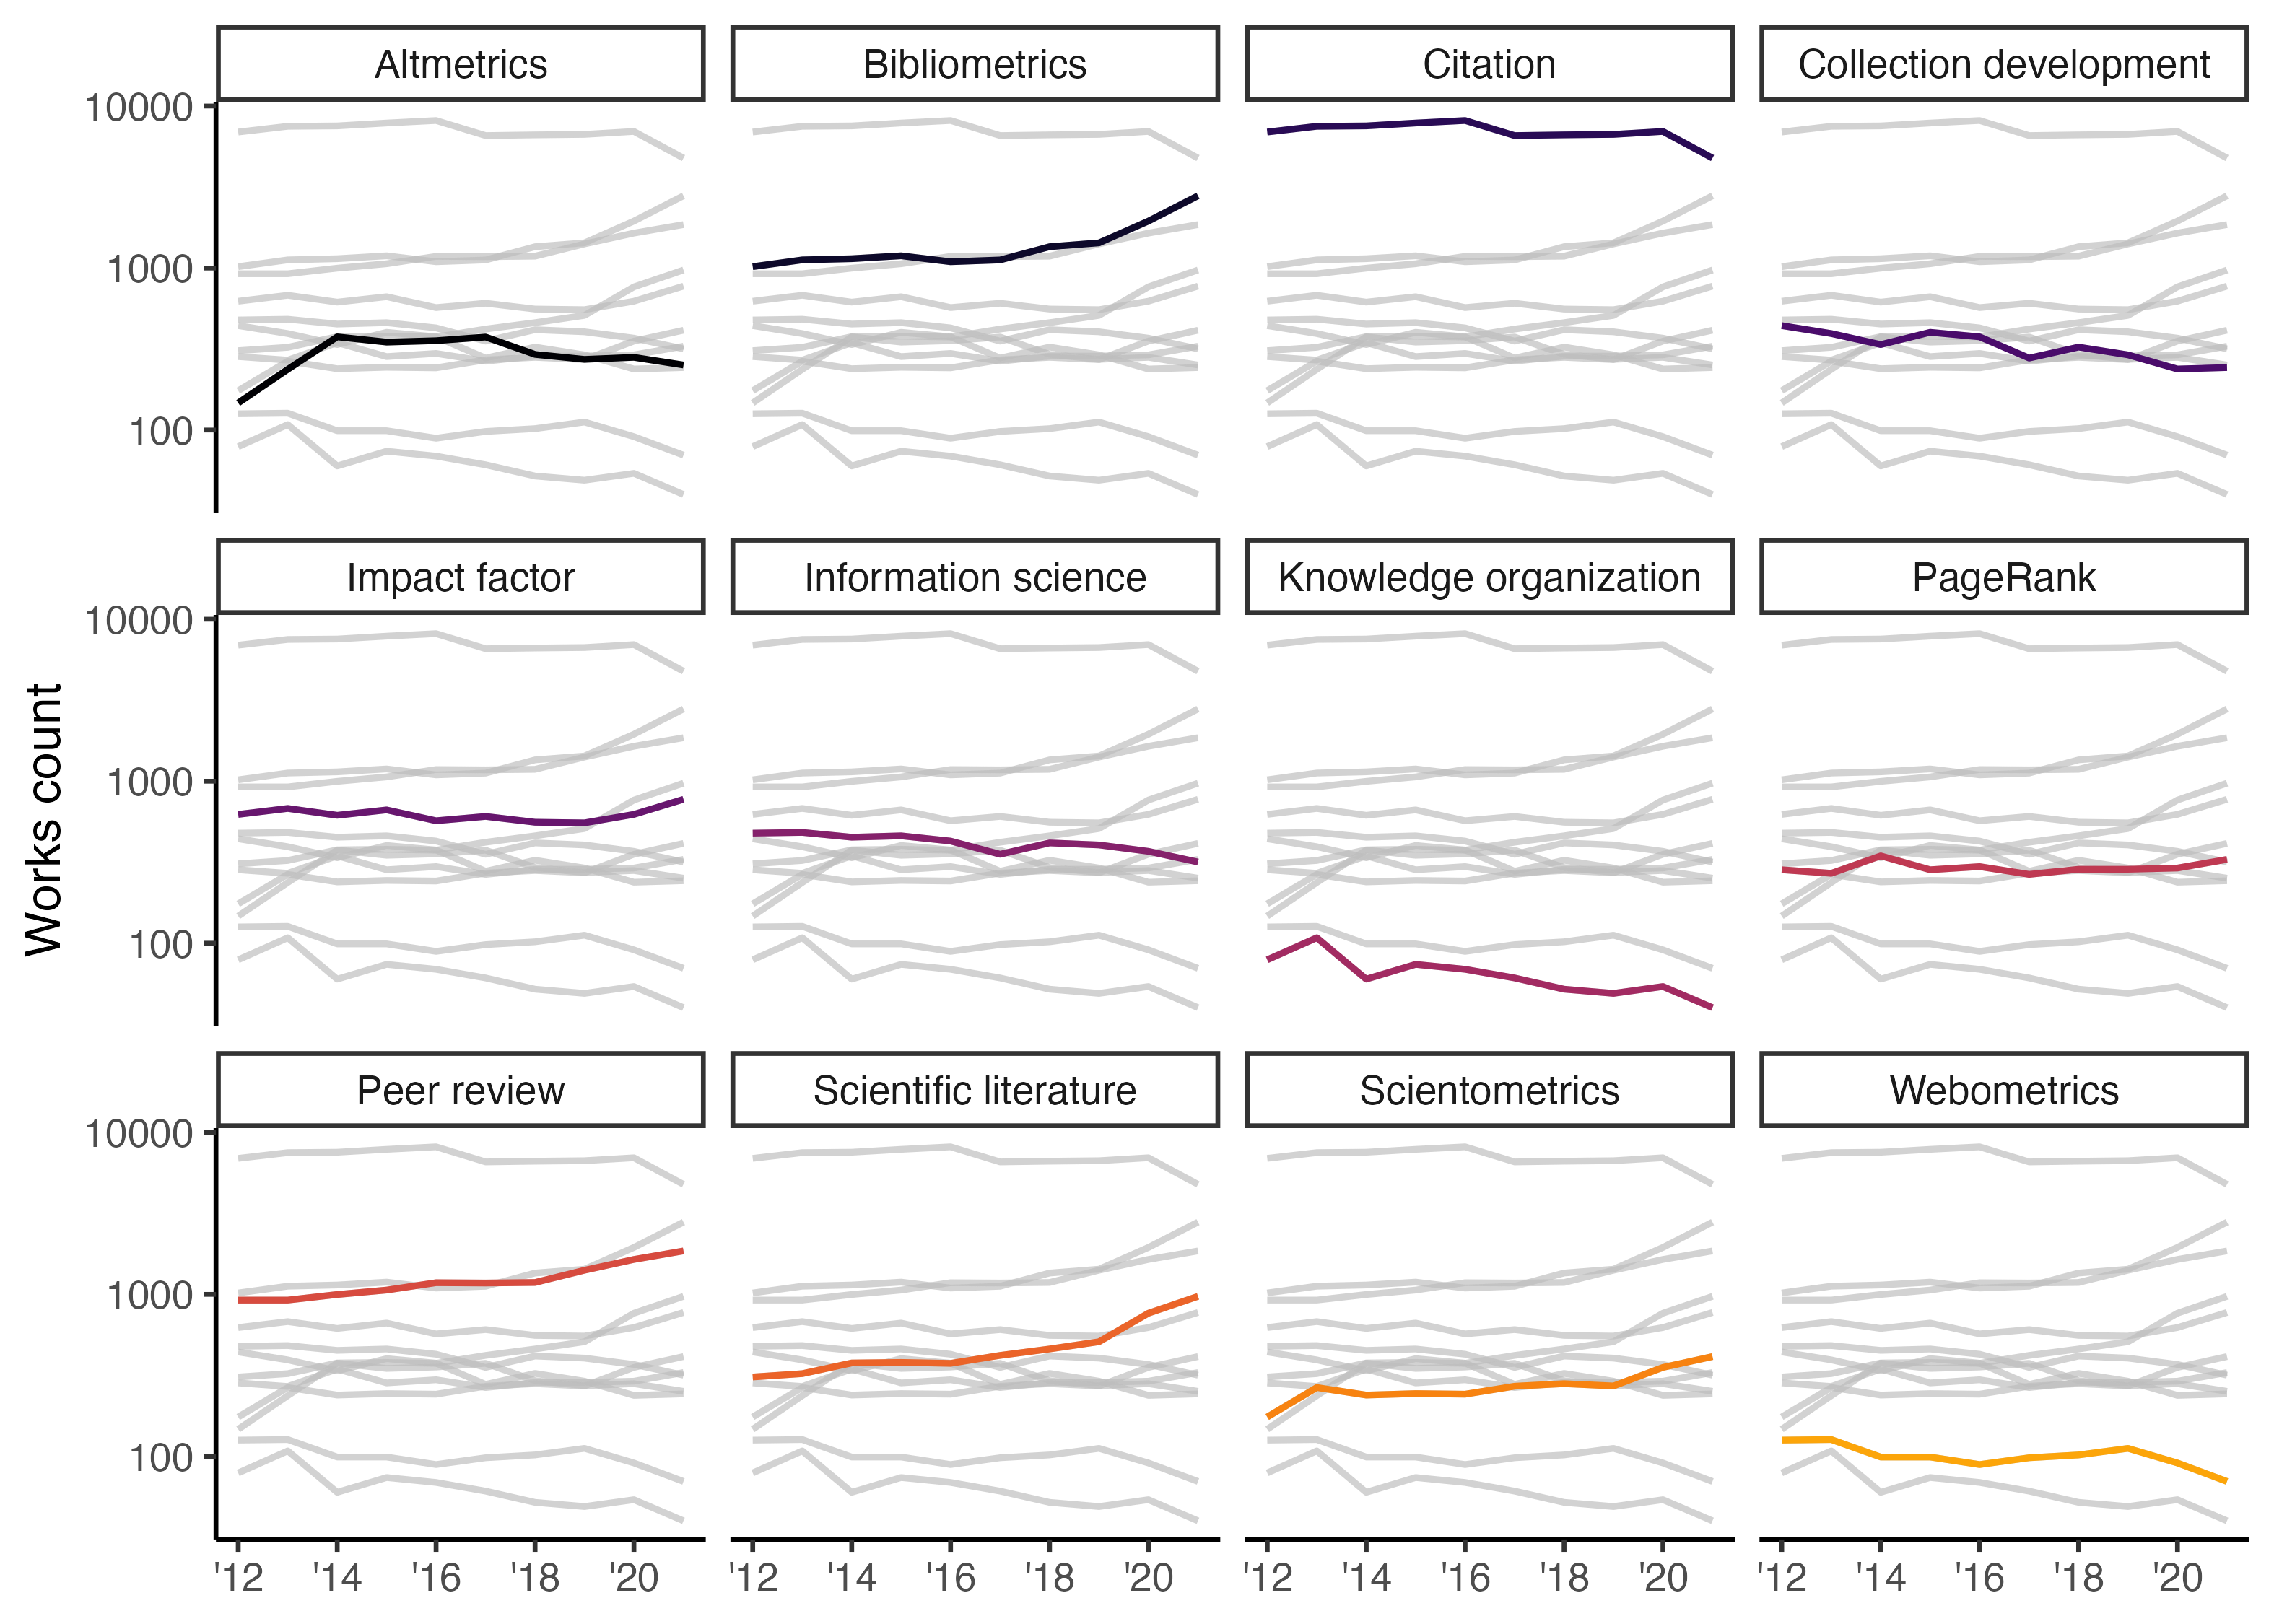
\includegraphics[scale=0.75]{figures/biblio-concepts}
  \caption{Trends in \emph{bibliometrics}-related topics in the past 10 years.}
  \label{bibli_concepts}
\end{figure}

\subsection{\emph{Bibliometrics} dataset}
We download all works, included in OpenAlex, that have the words \emph{bibliometrics} or \emph{science mapping} in the title to map bibliometric approaches in the scientific literature.
We set the query using the following parameters: \code{entity} is "works"; \code{title.search} is \code{"bibliometrics|science mapping"} and, for the first part, \code{count\_only} is \code{TRUE} so we can see how many records will be returned.

\begin{example}
oa_fetch(
  entity = "works",
  title.search = "bibliometrics|science mapping",
  count_only = TRUE
)
#      count db_response_time_ms page per_page
# [1,] 26,953                118    1        1

biblio_works <- oa_fetch(
  entity = "works",
  title.search = "bibliometrics|science mapping",
  count_only = FALSE
)
\end{example}

Our query returns 26,953 works concerning bibliometrics.
By default, the \code{oa\_fetch} converts these records in a tibble object (dataframe) with each row containing information about a work.
This dataframe has 28 columns containing important information about a work, such as the publication date, DOI, reference works, and so on.
If users wish to convert the original nested list into another object, they can change the parameters in the following way \code{oa\_fetch(...,\ output = "list")}.
From this dataset, we could describe the most relevant sources, authors, and institutions.




\subsection{Most relevant sources }

We first identify the core journals for the discipline by tallying all bibliometrics-related works for each source and selecting the top 5 sources with the most works.


\begin{example}
sources <- biblio_works |>
  dplyr::count(so) |>
  tidyr::drop_na(so) |>
  dplyr::slice_max(n, n = 5) |>
  dplyr::pull(so)
  
sources
# [1] "Scientometrics"                                       
# [2] "Sustainability"  
# [3] "Social Science Research Network"                      
# [4] "International Journal Environmental Research and Public Health"                                        
# [5] "Environmental Science and Pollution Research"                                            
                           
\end{example}

Visualising these counts over the years (Fig.\ref{biblio_journals}), we observe the field has expanded overall, especially starting around 2015.
\emph{Scientometrics} is the oldest journal publishing on bibliometrics and remains the top source for these articles.
Other journals started to publish these works in 2015 and have maintained some volume in this field.
\emph{Sustainability} only started publishing in this field in 2017 but has rapidly increased its number of publications since.
In 2021, it was the second source to have published the most bibliometrics articles, after \emph{Scientometrics}.

\begin{figure}[htbp]
  \centering
  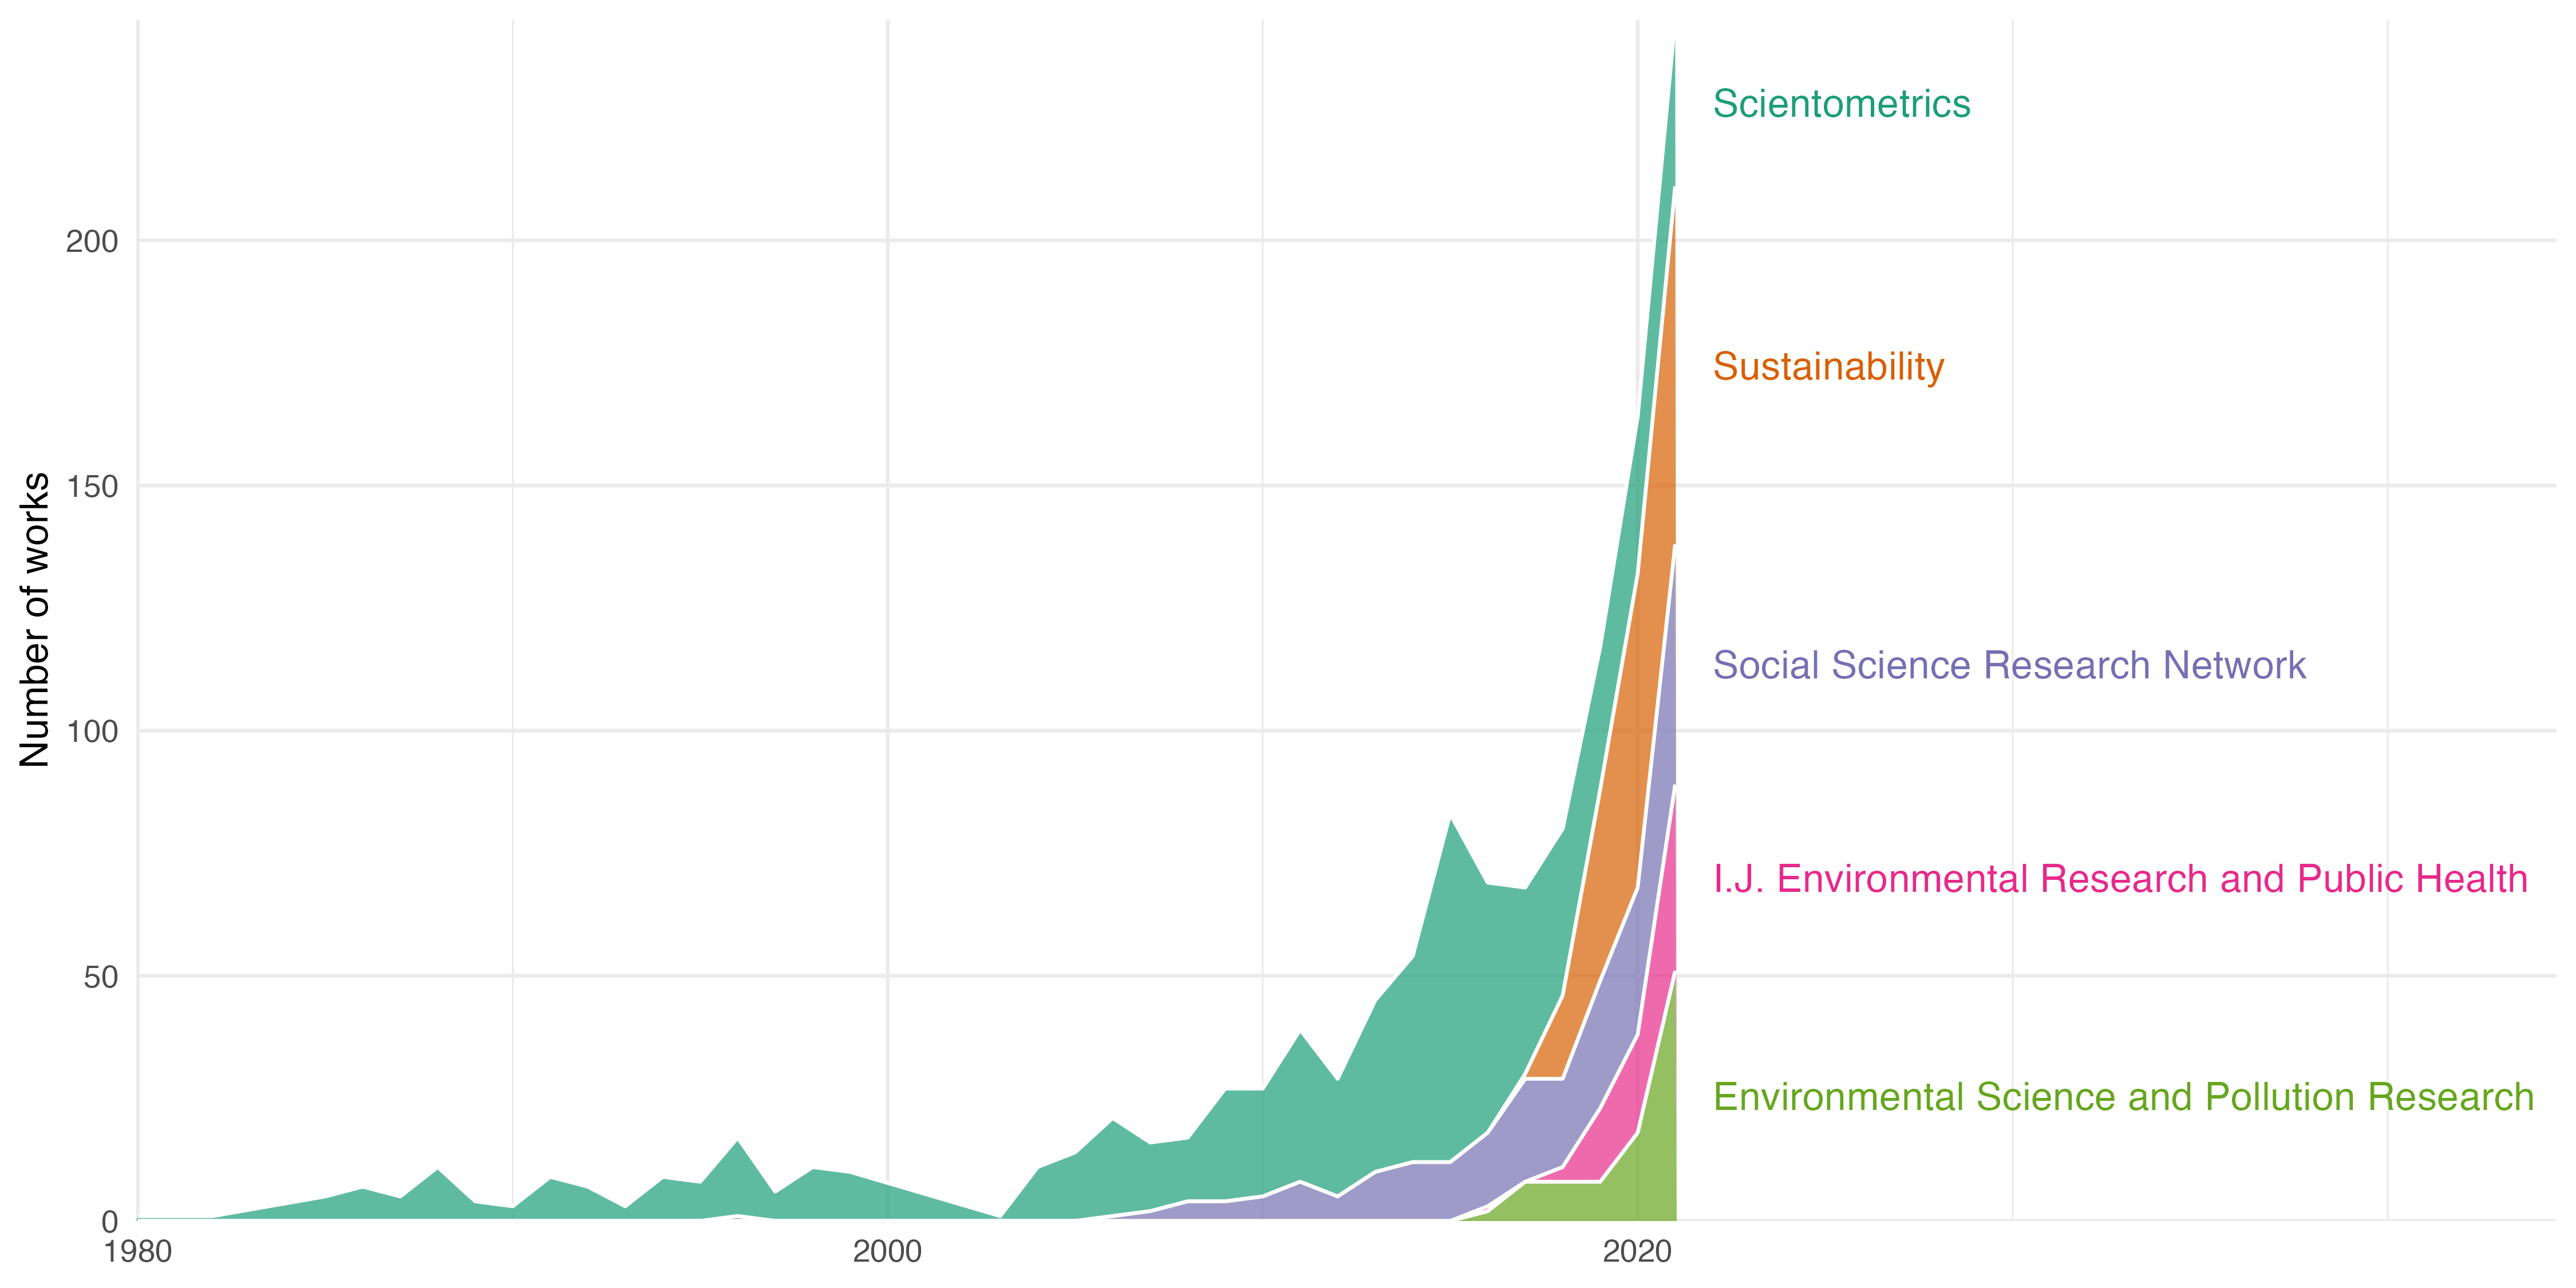
\includegraphics[scale=0.6]{figures/biblio-journals}
  \caption{Number of \emph{bibliometrics} articles by journal over the years.}
  \label{biblio_journals}
\end{figure}




\subsection{Most relevant authors and institutions}
Secondly, we identify the authors and institutions most relevant to the discipline by extracting the list of author and institution-related metadata from the collection, tallying all bibliometrics-related works for each author, and selecting the top 10 authors who write the most articles and 10 institutions with the most publications in the field.


\begin{example}
biblio_authors_raw <- do.call(rbind.data.frame, biblio_works$author)
biblio_insts <- biblio_authors_raw |>
  dplyr::count(institution_display_name) |>
  dplyr::rename("name" = institution_display_name) |>
  tidyr::drop_na(name) |>
  dplyr::slice_max(n, n = 10) |>
  dplyr::mutate(type = "Institution")

biblio_authors <- biblio_authors_raw |>
  dplyr::count(au_display_name) |>
  dplyr::rename("name" = au_display_name) |>
  tidyr::drop_na(name) |>
  dplyr::slice_max(n, n = 10) |>
  dplyr::mutate(type = "Author")
\end{example}

\begin{figure}[htbp]
  \centering
  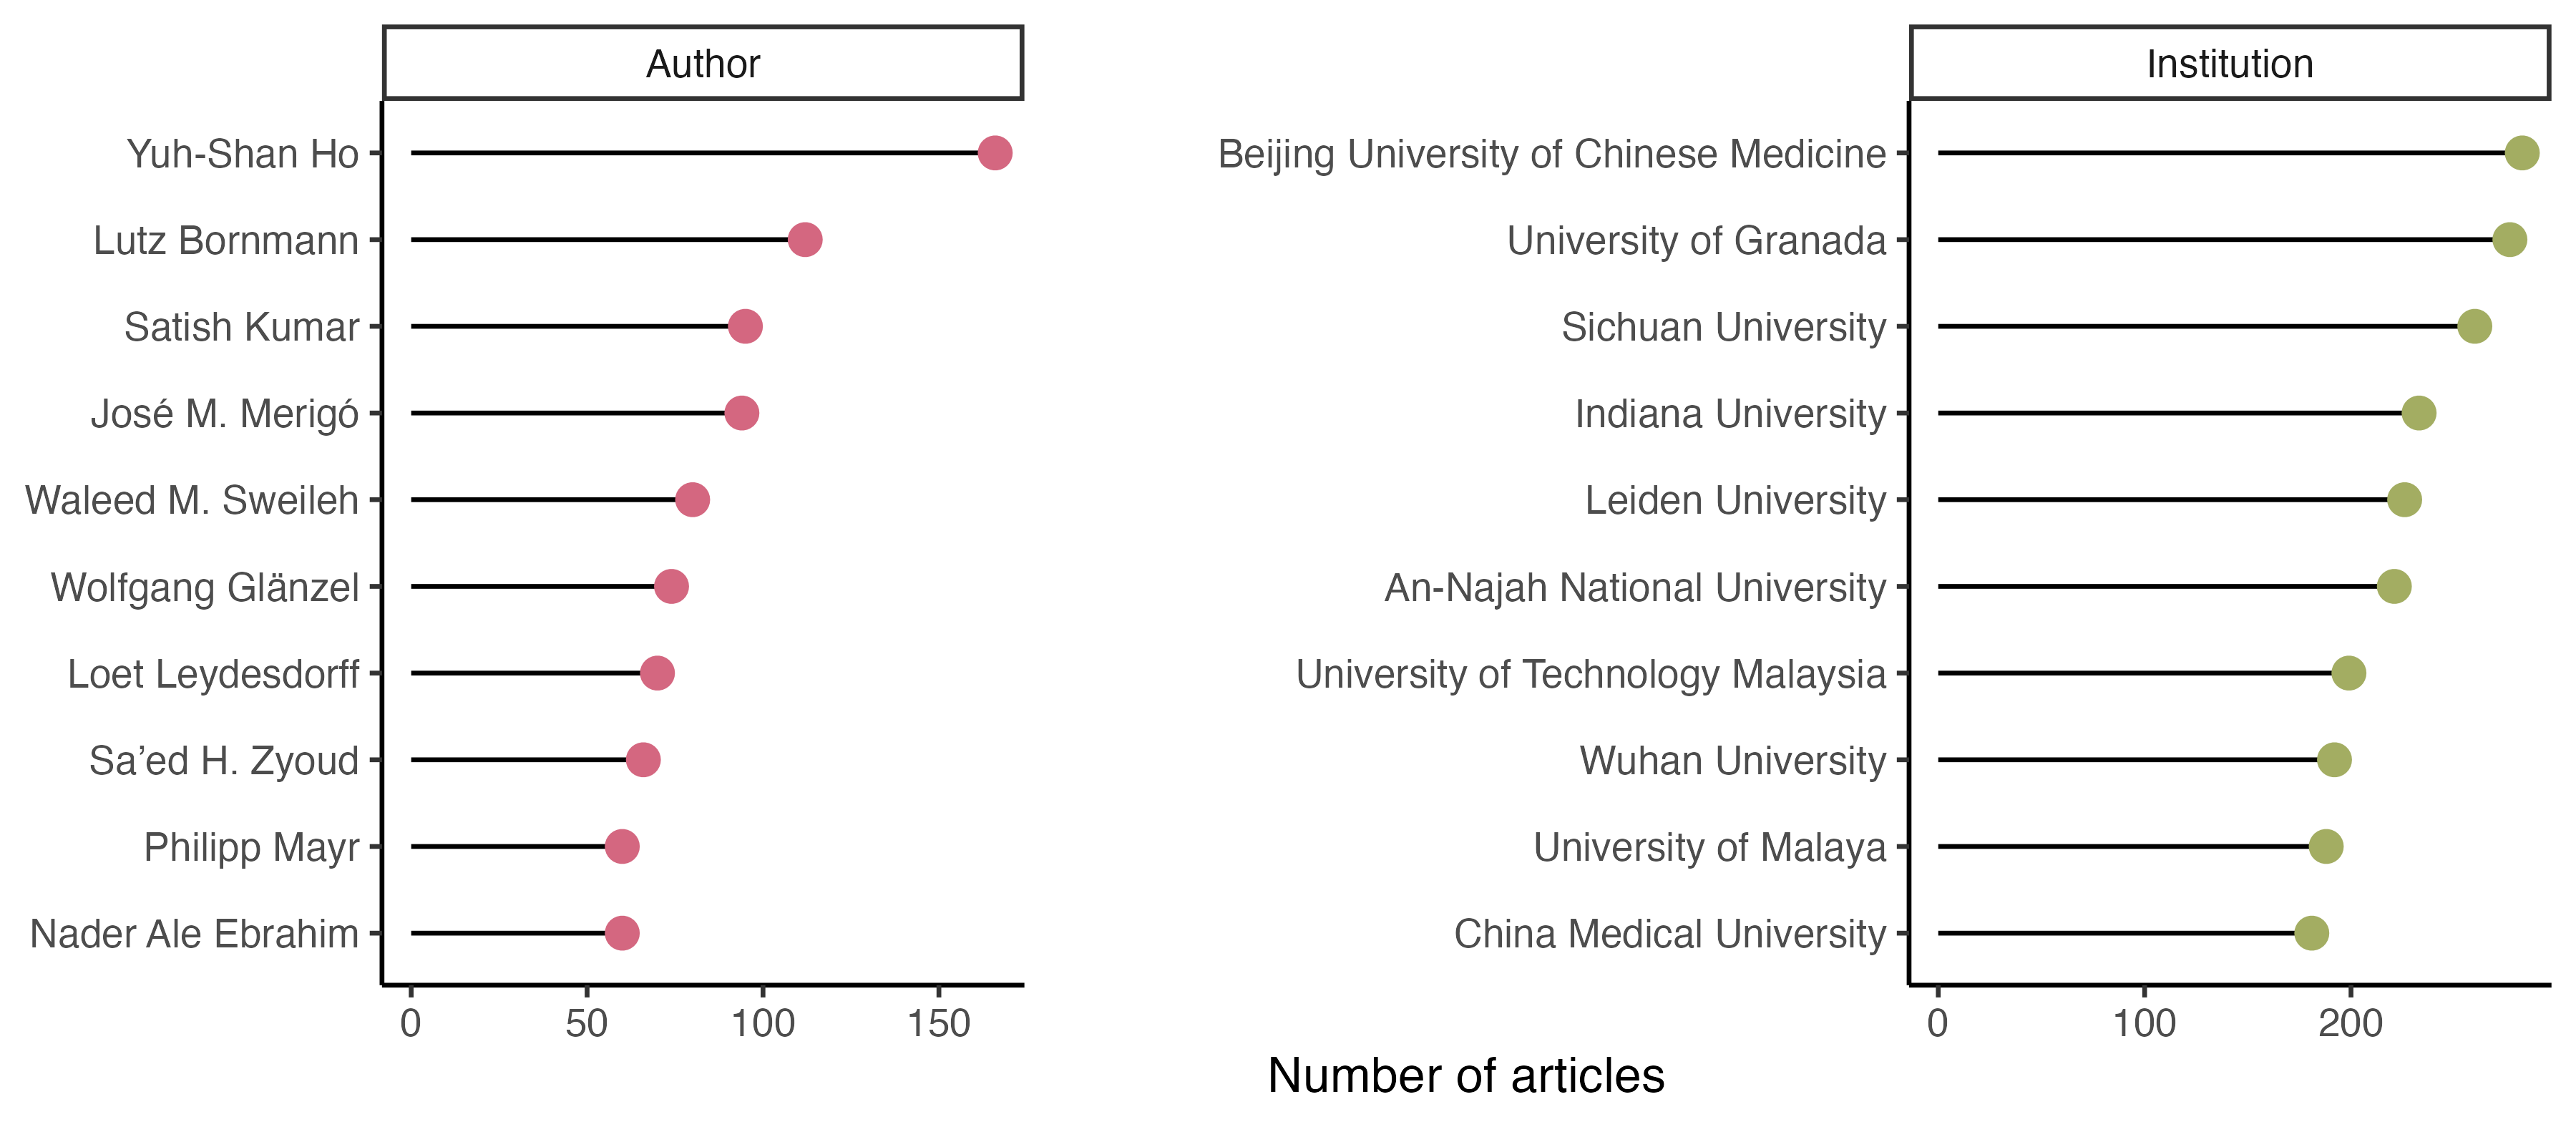
\includegraphics[scale=0.7]{figures/biblio-authors-institutions}
  \caption{Most relevant authors and institutions.}
  \label{mra}
\end{figure}

Among the 84,335 authors in our collection, Yuh-Shan Ho appears to have published the most bibliometrics articles. 
He has over 150 bibliometric papers in his career. 
Another relevant author in our collection is Lutz Bornmann with more than 100 bibliometrics papers. 
The other authors in the top 10 all have between 50 and 100 papers (Fig. \ref{mra}).

With regard to institutions, we observe that the concept \emph{bibliometrics} is widely developed by different centres of expertise. 
At the top of the ranking, we see Beijing University of Chinese Medicine (China) and University of Granada (Spain) with over 250 articles. 
Other relevant institutions in our dataset include Sichuan University (China), Indiana University (US), Leiden University (Netherlands), An-Najah National University (Palestine) with more than 200 bibliometric papers. 
Other institutions in the top 10 have between 150 and 200 papers (Fig.\ref{mra}).


\subsection{Most relevant works}

We identify the most relevant papers for the discipline by tallying all citations of articles related to bibliometrics and selecting the top 10 most cited articles (Tab.\ref{tab:mrp}).
We find 'Software survey: VOSviewer, a computer programme for bibliometric mapping' at the top with 4805 citations. 
Other relevant works in our collection are 'Comparison of PubMed, Scopus, Web of Science, and Google Scholar: strengths
and weaknesses' with 1996 citations and 'bibliometrix: An R-tool for comprehensive science mapping analysis' with 1800 citations. The other papers in the top 10 all have between 950 and 1500 citations.

\begin{example}
seminal_works <- slice_max(biblio_works, cited_by_count, n = 10)

# output in Table 2:
seminal_works |>
  dplyr::select(publication_date, display_name, so, cited_by_count)  
\end{example}

\begin{table}[!ht]
\begin{footnotesize}
    \begin{tabular}{llll}
        Year & Article & source & Cited \\ \hline
        2010 & Software survey: VOSviewer,  & Scientometrics & 5364 \\ 
        ~ & a computer program for bibliometric mapping & ~ & ~ \\ 
        2017 & bibliometrix : An R-tool for  & Journal of Informetrics & 2127 \\ 
        ~ & comprehensive science mapping analysis & ~ & ~ \\ 
        1976 & A general theory of bibliometric  & Journal of the American Society  & 1505 \\ 
        ~ & and other cumulative advantage processes & for Information Science & ~ \\ 
        2015 & Bibliometric Methods in Management and  & Organizational Research Methods & 1488 \\ 
        ~ & Organization & ~ & ~ \\ 
        2015 & Bibliometrics: The Leiden Manifesto for research metrics & Nature & 1168 \\ 
        2011 & Science mapping software tools: Review, analysis,  & Journal of the Association for & 1100 \\ 
        ~ & and cooperative study among tools &  Information Science and Technology & ~ \\ 
        2004 &  Changes in the intellectual structure of strategic  & Strategic Management Journal & 1038 \\ 
        ~ & management research: a bibliometric study  & ~ & ~ \\ 
        ~ & of the Strategic Management Journal, 1980–2000 & ~ & ~ \\ 
        2010 & A unified approach to mapping & Journal of Informetrics & 922 \\ 
        ~ &  and clustering of bibliometric networks & ~ & ~ \\ 
        2015 & Green supply chain management:  & International Journal of  & 920 \\ 
        ~ & A review and bibliometric analysis & Production Economics & ~ \\ 
        2006 & Forecasting emerging technologies:  & Technological Forecasting  & 804 \\ 
        ~ & Use of bibliometrics and patent analysis & and Social Change & ~ \\ 
    \end{tabular}
    \end{footnotesize}
    \caption{Most relevant works}
    \label{tab:mrp}
    \end{table}


\subsection{Snowball search}
We perform snowballing with \code{oa\_snowball} to identify the set of articles that cite and are cited by the two seminal works associated with the concept of bibliometrics: Software survey: VOSviewer, a computer programme for bibliometric mapping (W2150220236), bibliometrix : An R-tool for comprehensive science mapping analysis (W2755950973).
We insert these OAIDs as identifiers in \code{oa\_snowball}, use the filter on the citations obtaining only those related to 2022, then use \CRANpkg{tidygraph} \citep{tidygraph} and \CRANpkg{ggraph} \citep{ggraph} to display this citation network (Fig. \ref{citation_graph}). \code{oa\_snowball} returns a list of 2 elements: nodes and edges. The first have information about the work, while edges have the start and end points of the links. 
This list output from \code{oa\_snowball} can be used directly as input to standard graph functions such as \code{tidygraph::as\_tbl\_graph} for further network analyses and visualisations in co-citation analysis, historiograph analysis, \emph{etc.}



\begin{example}
sb_docs <- oa_snowball(
  identifier = c("W2150220236", "W2755950973"),
  citing_filter = list(from_publication_date = "2022-01-01")
)

# Reduced output
print(sb_docs)
$nodes
# A tibble: 5,769 × 37
  id          display_name                        
  <chr>       <chr>                               
1 W2150220236 Software survey: VOSviewer, a computer program for bibliometric ...               
2 W2755950973 bibliometrix : An R-tool for comprehensive science mapping analysis                   
3 W4306178549 Literature reviews as independent studies: guidelines for academic ...           
4 W4320070415 Is Metaverse in education a blessing or a curse: a combined content  ...
# i 5,765 more rows
# i 35 more variables
$edges
# A tibble: 6,444 × 2
  from        to         
  <chr>       <chr>      
1 W4306178549 W2755950973
2 W4320070415 W2150220236
3 W3203542139 W2150220236
4 W4283392904 W2150220236
# i 6,440 more rows

# Conversion to a `tbl_graph` object for network analysis and visualization
sb_docs_graph <- tidygraph::as_tbl_graph(sb_docs)
\end{example}


\begin{figure}[htbp]
  \centering
  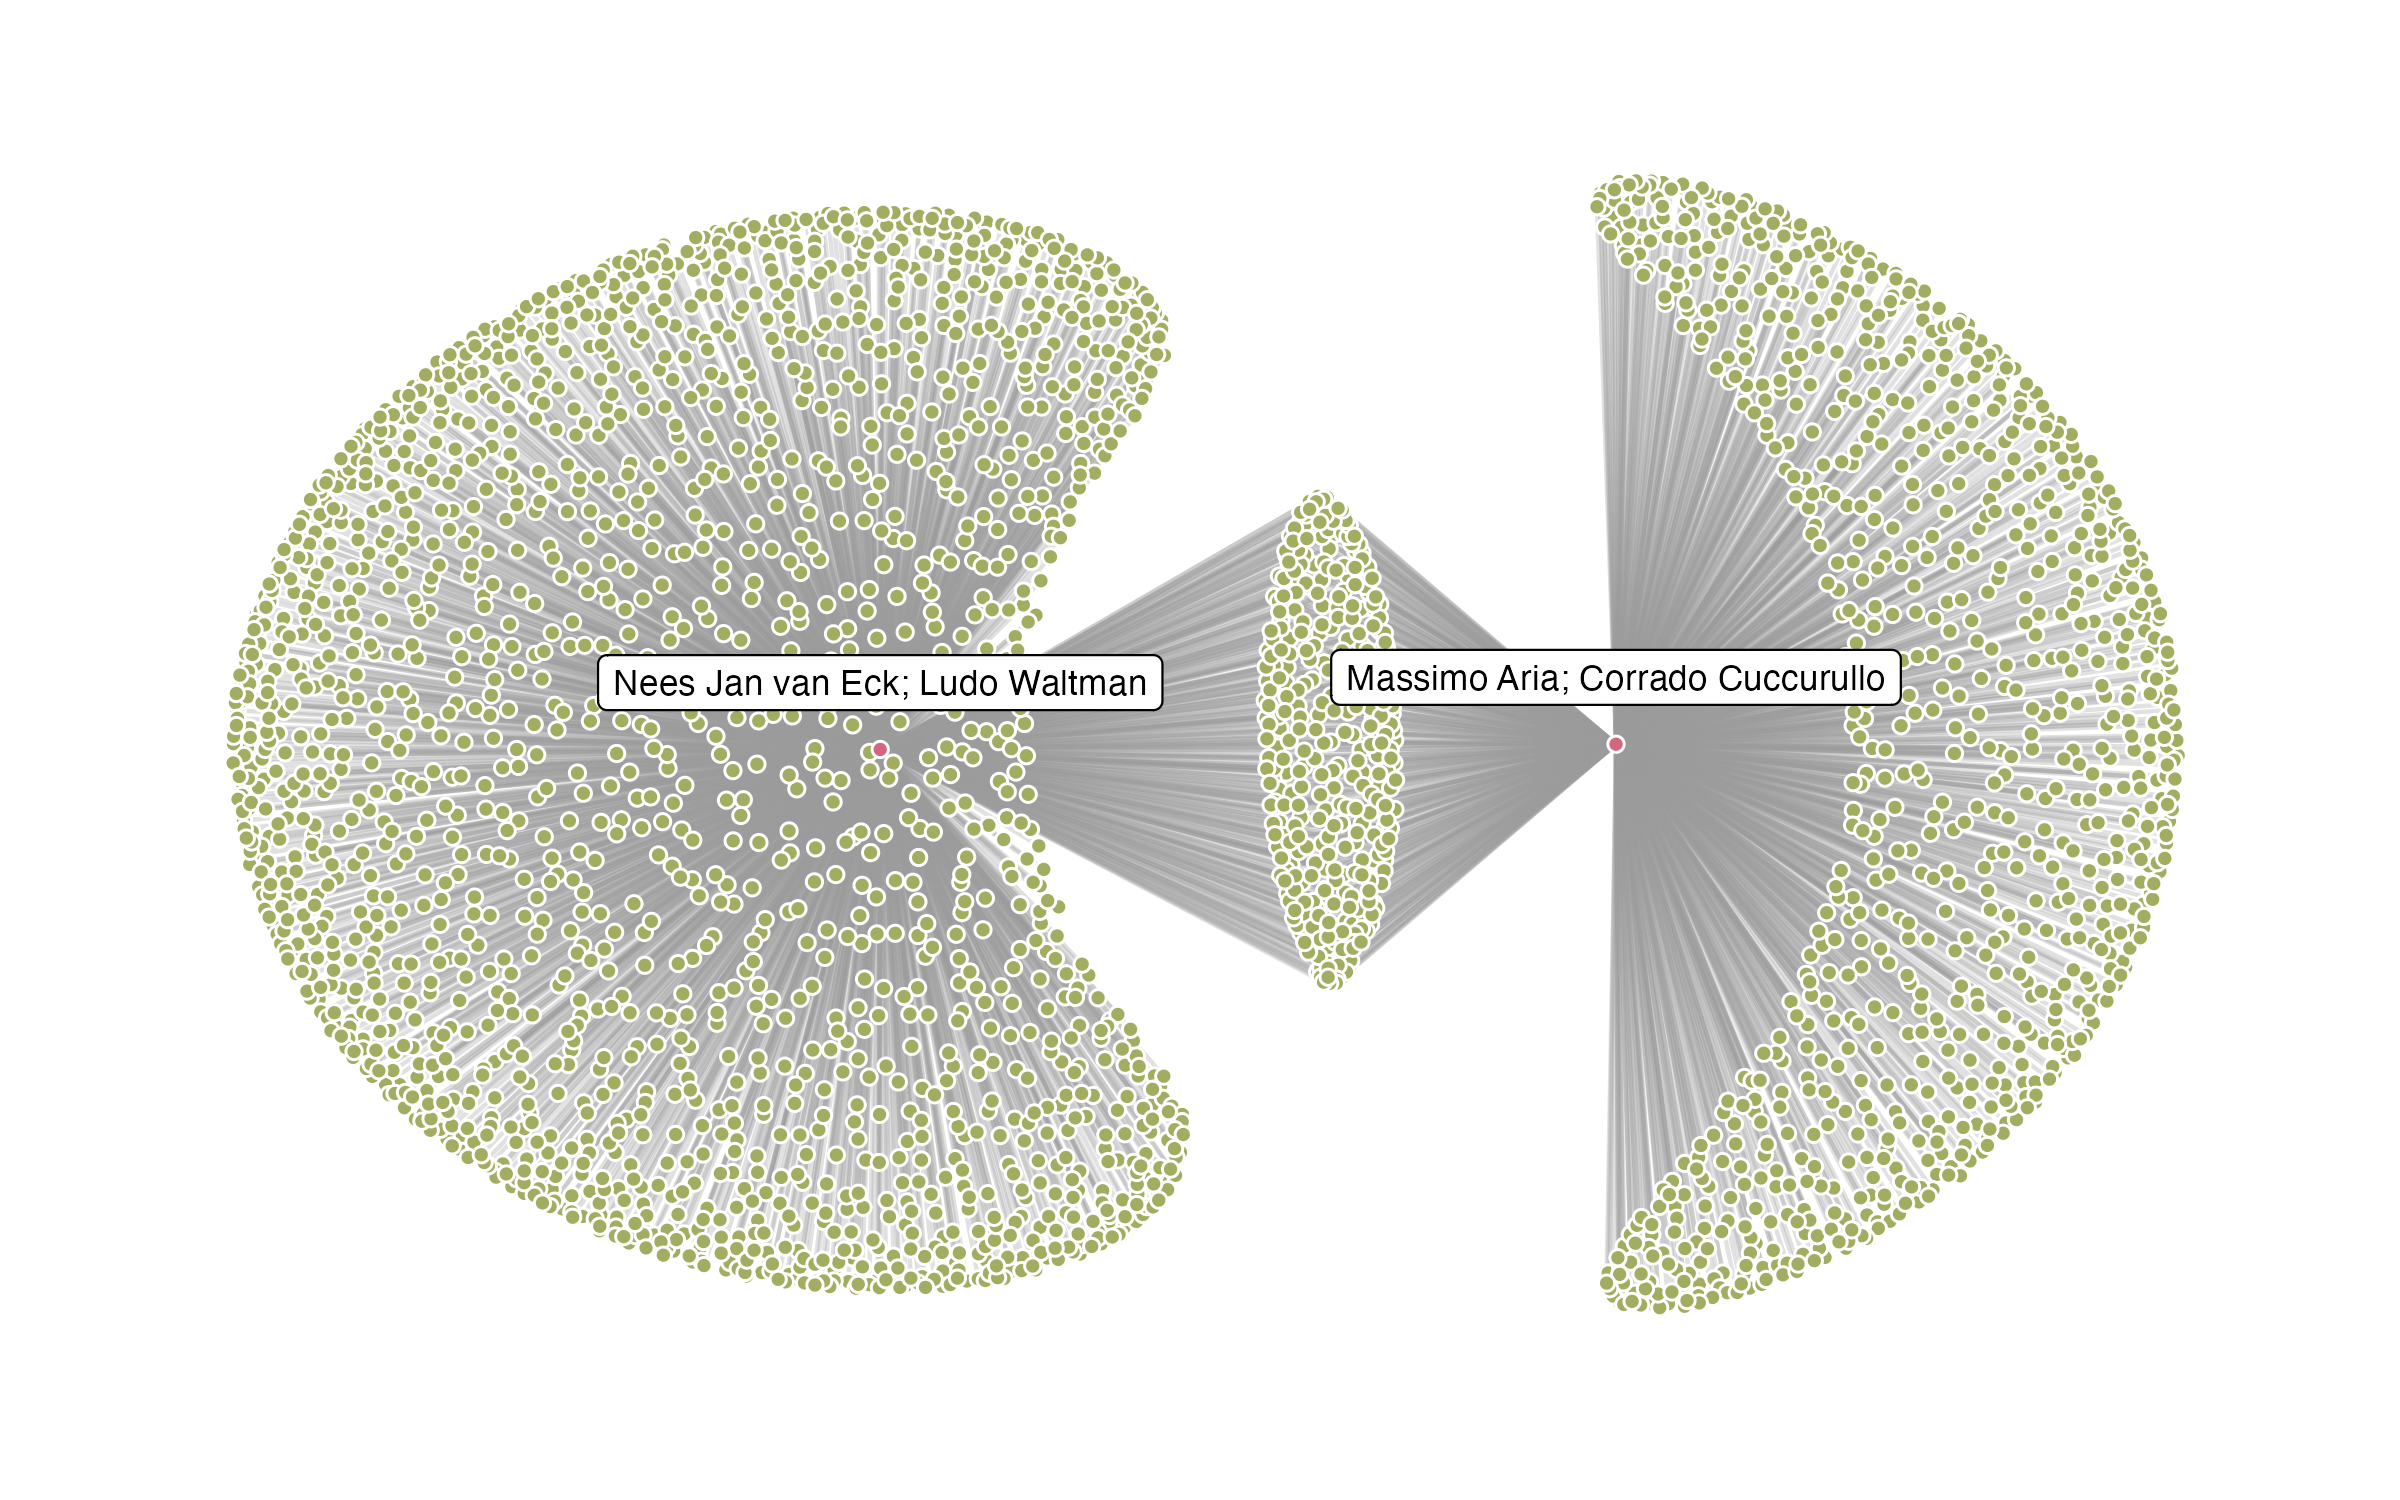
\includegraphics[scale=0.72]{figures/citation-graph}
  \caption{Two seminal works and their citations and references, from \code{oa\_snowball} output.}
  \label{citation_graph}
\end{figure}



\code{oa\_snowball} finds and returns the metadata on the two seminal works in our dataset, and also information on the articles that cite and are cited by them, in 2022. We have a total of 2,907 citing articles: 2,078 articles cite van Eck et al., 1,161 articles cite Aria and Cuccurullo. In addition, as we can see from the graph, there are 332 articles citing both van Eck et al. and Aria and Cuccurullo, simultaneously.


\subsection{N-grams}

Finally, we obtain the N-grams of all the bibliometric works that make up our collection. N-grams are groups of words that occur in the full text of a work. To extract n-grams we use the \code{oa\_ngrams} function from the \pkg{openalexR} package. From this list we then extract only the bigrams because we believe they can be more informative.

\begin{example}
ngrams_data <- oa_ngrams(sample(biblio_works$id, 1000), verbose = TRUE)
top_10 <- do.call(rbind.data.frame, ngrams_data$ngrams) |>
  dplyr::filter(ngram_tokens == 2, nchar(ngram) > 10) |>
  dplyr::arrange(desc(ngram_count)) |>
  dplyr::slice_max(ngram_count, n = 10, with_ties = FALSE)
\end{example}

\begin{figure}[htbp]
  \centering
  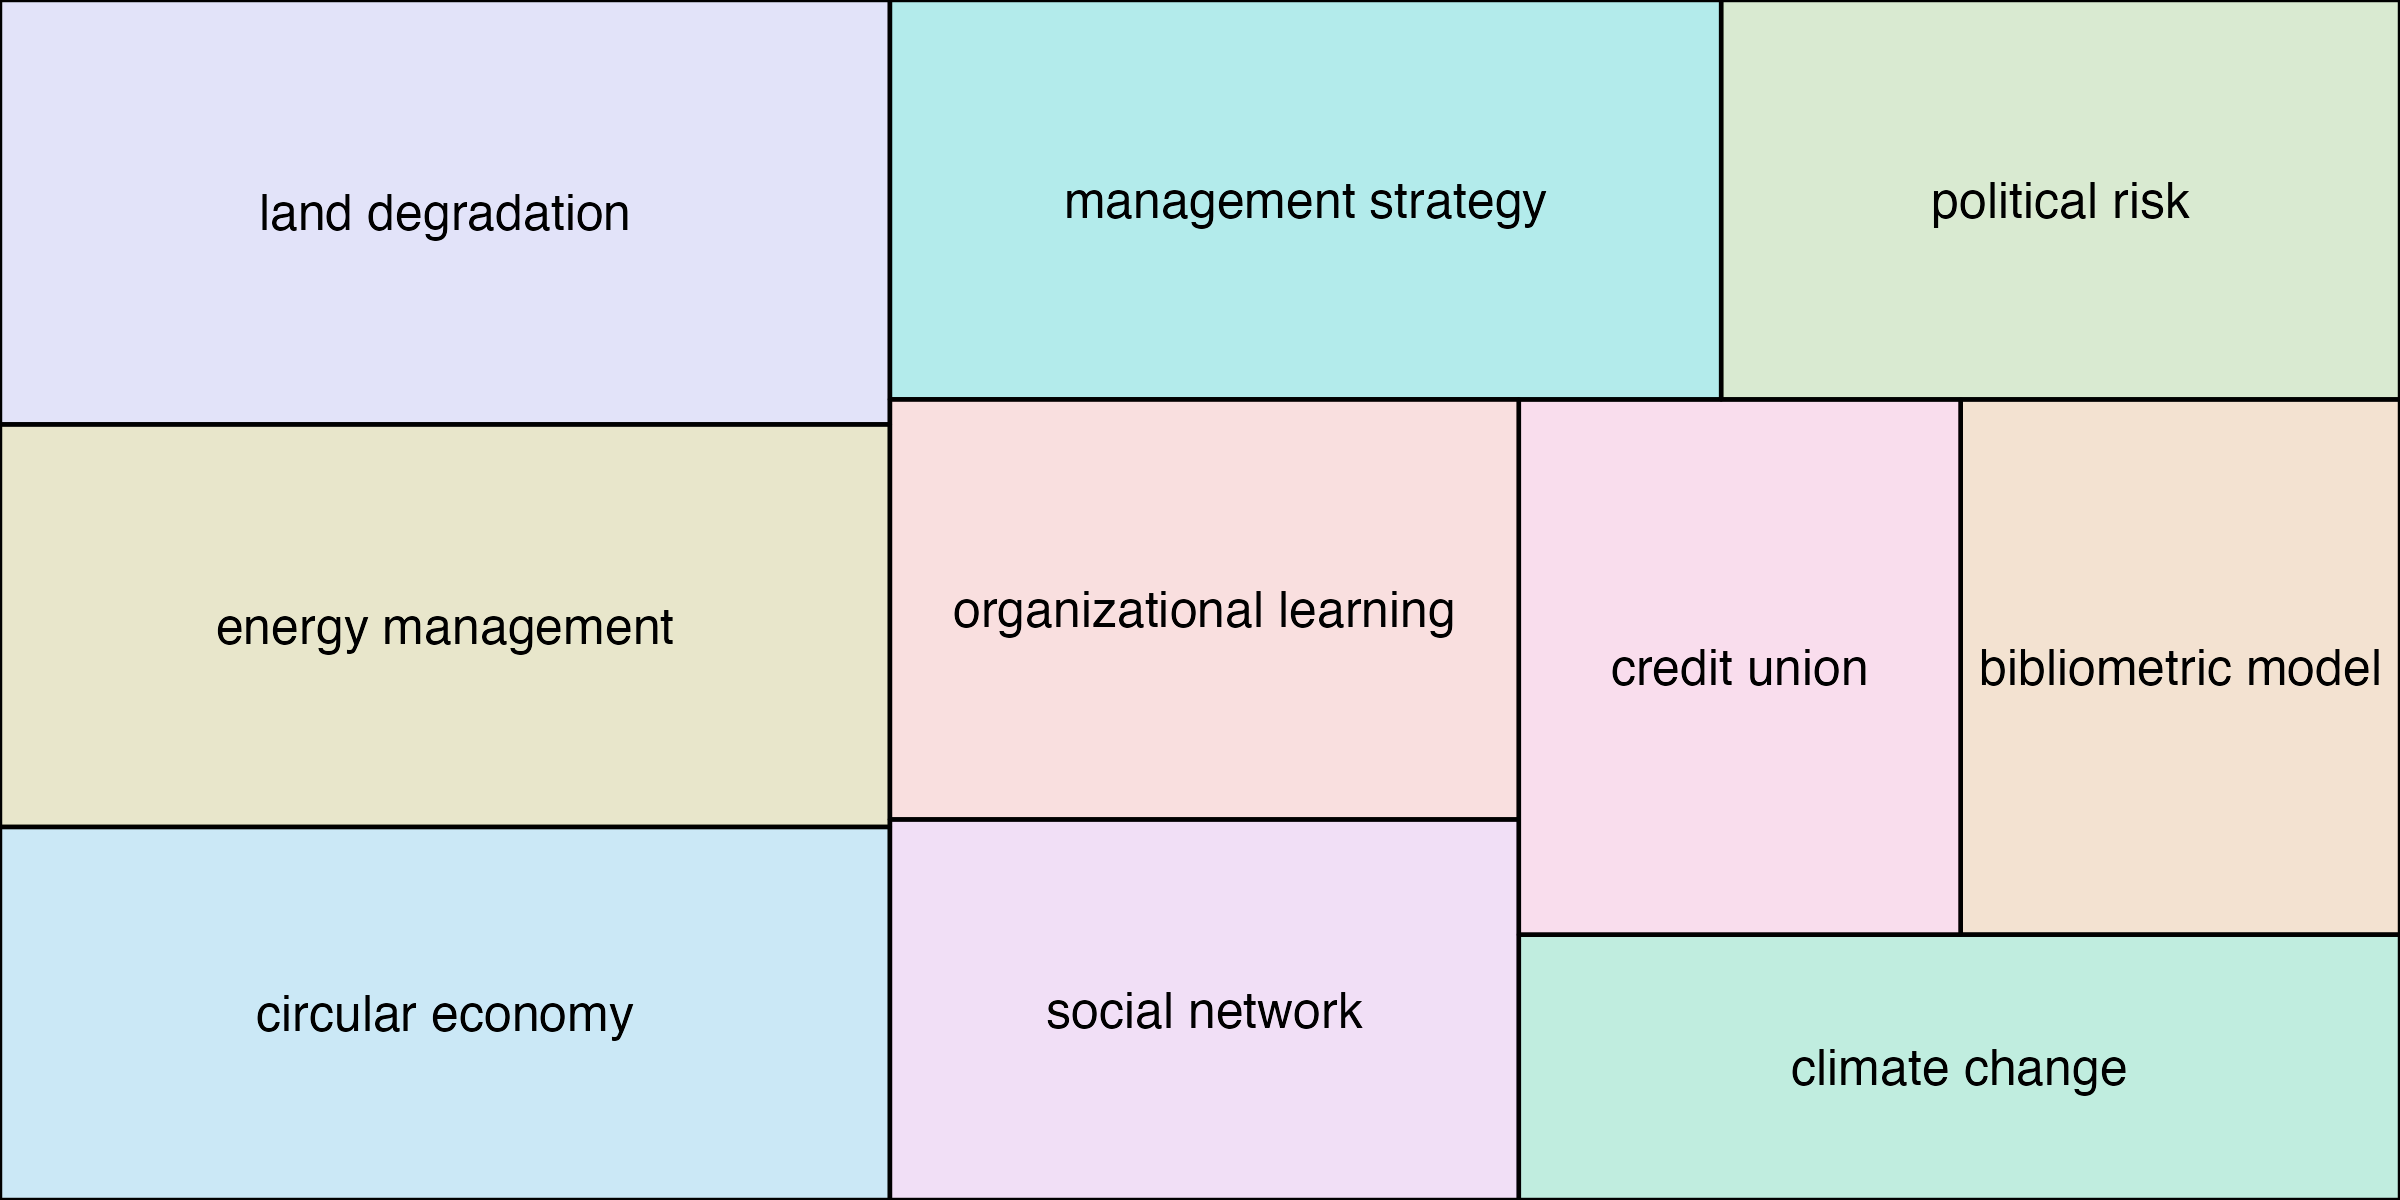
\includegraphics[scale=0.6]{figures/ngram-treemap}
  \caption{TreeMap of the top 10 bi-grams of \emph{bibliometrics} articles.}
  \label{treemap}
\end{figure}

As can be seen from the graph of the 10 most frequent bi-grams, the papers are very much focused on the use of advanced technologies to improve efficiency and sustainability in various fields, such as \emph{circular economy}, \emph{climate change}, \emph{management strategy}, and \emph{energy management} (Fig. \ref{treemap}).
In addition, there are themes related to \emph{political risk}, \emph{organizational learning}, and cooperation within organizations and \emph{social networks}. 
In general, these topics suggest the need for greater attention to environmental and social issues in business management and risk prevention.
Finally, \emph{bibliometric model} (scientific performance evaluation) and \emph{credit union} (financial regulation) are interrelated to bibliometrics, which requires a global vision and cooperation among different stakeholders to be effectively applied. 

\section{Summary}
\pkg{openalexR} is a new package that facilitates querying, collecting, and downloading bibliographic metadata of OpenAlex entities through the provided REST APIs.
It is available on CRAN at \url{https://cran.r-project.org/package=openalexR}.
\pkg{openalexR} helps streamline the researcher's workflow in accessing, collecting, and wrangling OpenAlex data.
Extensive documentation, comprehensive tests of the package's internal functions, and common use cases are provided, sufficiently covering the current OpenAlex API.
The source code and development versions are available at \url{https://github.com/ropensci/openalexR}.
The current version of the package is a stable version, and there are no plans for any breaking changes soon.
Of course, \pkg{openalexR} will continue to be actively maintained to keep up with CRAN policies and distribute any bug fixes.
Bug reports, help requests, or improvement suggestions are welcome in the package software repository.
For more information on \pkg{openalexR}, vignettes are available at \url{https://ropensci.github.io/openalexR/articles/}.


\section{Acknowledgements}

\section{Supplementary material}

Examples we show in this manuscript can be found at \url{https://github.com/trangdata/oarj/blob/main/paper-examples.md}.

